\documentclass[12pt,a4paper]{report}
\usepackage[utf8]{inputenc}
\usepackage{graphicx}
\usepackage{float}
\usepackage{hyperref}
\usepackage{amsmath}
\usepackage{algorithm}
\usepackage{algpseudocode}
\usepackage{tikz}
\usetikzlibrary{shapes.geometric, arrows.meta, positioning, fit, backgrounds, calc, shadows}
\usepackage{listings}
\usepackage{xcolor}
\usepackage{booktabs}
\usepackage{caption}
\usepackage{subcaption}
\usepackage{multirow}
\usepackage[margin=1in]{geometry}

% Define colors for code listings
\definecolor{codegreen}{rgb}{0,0.6,0}
\definecolor{codegray}{rgb}{0.5,0.5,0.5}
\definecolor{codepurple}{rgb}{0.58,0,0.82}
\definecolor{backcolour}{rgb}{0.95,0.95,0.92}

%% ── Dissertation-appropriate colour definitions (keeping original blue!20) ──
\definecolor{nodeblue}{rgb}{0.678,0.847,0.902}   % blue!20 equivalent
\definecolor{nodeborder}{rgb}{0.0,0.447,0.698}   % professional deep blue border
\definecolor{arrowgrey}{rgb}{0.2,0.2,0.2}        % near-black for main arrows
\definecolor{feedbackred}{rgb}{0.72,0.11,0.11}   % deep academic red
\definecolor{borderbox}{rgb}{0.3,0.3,0.3}        % outer dashed border

\lstdefinestyle{mystyle}{
    backgroundcolor=\color{backcolour},   
    commentstyle=\color{codegreen},
    keywordstyle=\color{magenta},
    numberstyle=\tiny\color{codegray},
    stringstyle=\color{codepurple},
    basicstyle=\ttfamily\footnotesize,
    breakatwhitespace=false,         
    breaklines=true,                 
    captionpos=b,                    
    keepspaces=true,                 
    numbers=left,                    
    numbersep=5pt,                  
    showspaces=false,                
    showstringspaces=false,
    showtabs=false,                  
    tabsize=2
}
\lstset{style=mystyle}

\begin{document}

\chapter{Methodology}

\section{Introduction}
This chapter presents the comprehensive methodology employed in developing the Kiswahili Speech Analytics System. The methodology aligns with the research objectives outlined in Chapter 1, specifically addressing: (1) the development of an automated speech recognition (ASR) system for Kiswahili, (2) sentiment analysis of transcribed speech, and (3) deployment of a production-ready system for real-time audio processing.

The research adopts a software engineering approach combined with machine learning experimentation methodologies. This chapter details the systematic process followed from problem analysis through system deployment, including data preparation, model development, system architecture design, implementation, testing, and validation.

\section{Research Design}
\subsection{Overall Approach}
This research follows an applied research design with a focus on system development and empirical evaluation. The methodology integrates:

\begin{itemize}
    \item \textbf{Experimental Research}: For model training, evaluation, and optimization
    \item \textbf{Software Development Methodology}: Agile iterative approach for system implementation
    \item \textbf{Design Science Research}: Creating and evaluating artifacts (models and system)
\end{itemize}

The research questions stated in Chapter 1 are addressed through a combination of literature review (partially answering theoretical questions) and empirical system development (answering practical implementation questions).

\subsection{Software Development Methodology}
The project adopts an \textbf{Agile Development Methodology} with iterative cycles, allowing for continuous refinement based on model performance and system requirements. The choice of Agile is justified by:

\begin{itemize}
    \item Flexibility to adapt to model performance results
    \item Iterative improvement of machine learning models
    \item Rapid prototyping and testing capabilities
    \item Continuous integration of new features
\end{itemize}

Figure \ref{fig:agile_process} illustrates the iterative development process followed in this research.

\begin{figure}[H]
    \centering
    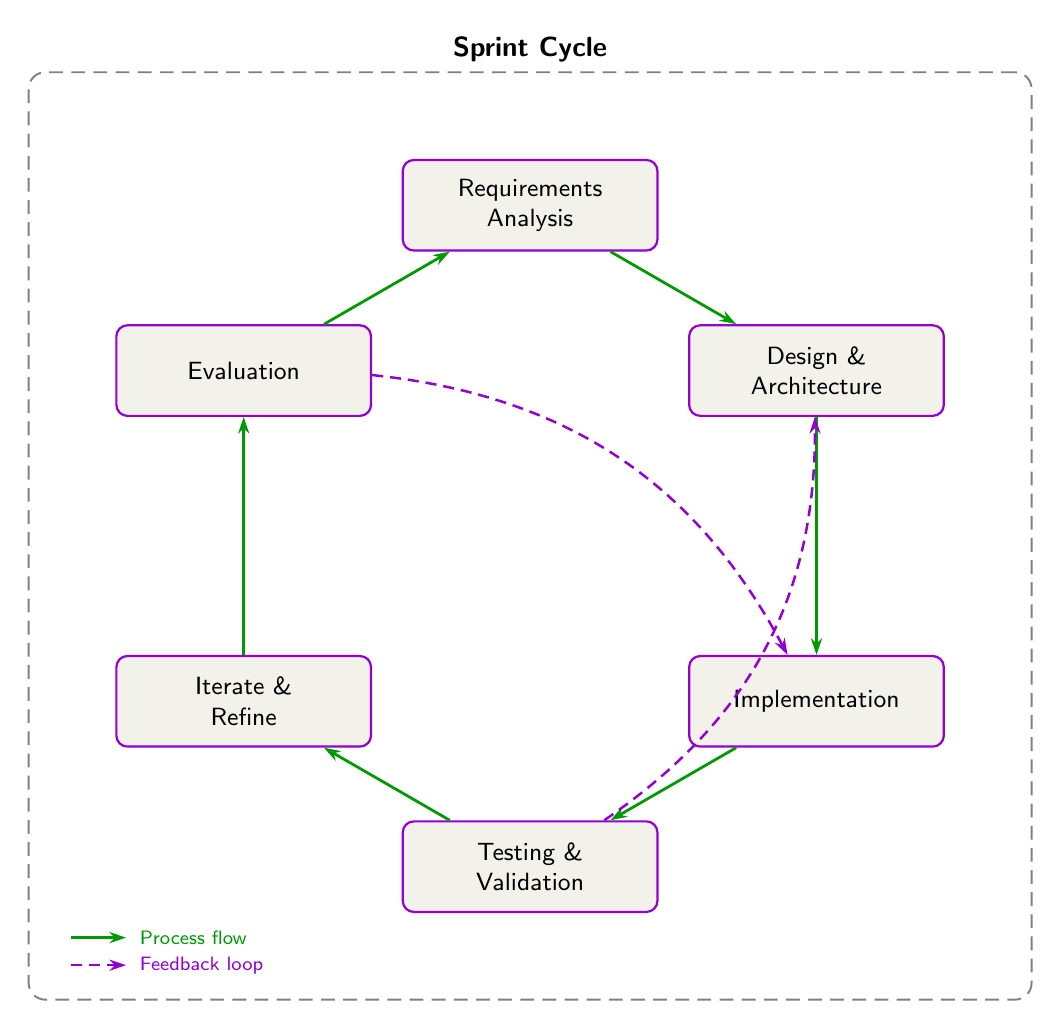
\begin{tikzpicture}[
    box/.style={
        rectangle,
        draw=codepurple,
        line width=0.8pt,
        fill=backcolour,
        text width=3.0cm,
        text centered,
        rounded corners=4pt,
        minimum height=1.15cm,
        font=\small\sffamily
    },
    arrow/.style={
        -{Stealth[length=6pt, width=4pt]},
        line width=1.0pt,
        color=codegreen
    },
    fbarrow/.style={
        -{Stealth[length=6pt, width=4pt]},
        line width=0.9pt,
        dashed,
        dash pattern=on 4pt off 2.5pt,
        color=codepurple
    }
]

\node[box] (req)     at (90:4.2cm)   {Requirements\\Analysis};
\node[box] (design)  at (30:4.2cm)   {Design \&\\Architecture};
\node[box] (impl)    at (-30:4.2cm)  {Implementation};
\node[box] (test)    at (-90:4.2cm)  {Testing \&\\Validation};
\node[box] (iterate) at (-150:4.2cm) {Iterate \&\\Refine};
\node[box] (eval)    at (150:4.2cm)  {Evaluation};

\draw[arrow] (req)     -- (design);
\draw[arrow] (design)  -- (impl);
\draw[arrow] (impl)    -- (test);
\draw[arrow] (test)    -- (iterate);
\draw[arrow] (iterate) -- (eval);
\draw[arrow] (eval)    -- (req);

\draw[fbarrow] (test) to[bend right=28] (design);
\draw[fbarrow] (eval) to[bend left=28]  (impl);

\node[
    draw=codegray,
    dashed,
    dash pattern=on 5pt off 3pt,
    line width=0.7pt,
    rounded corners=6pt,
    fit=(req)(design)(impl)(test)(iterate)(eval),
    inner sep=1.1cm,
    label={[font=\normalsize\sffamily\bfseries, color=black]above:Sprint Cycle}
] (boundary) {};

\begin{scope}[shift={($(boundary.south west)+(0.55cm,0.45cm)$)}]
    \draw[arrow, shorten >=0pt, shorten <=0pt] (0,0.35cm) -- (0.7cm,0.35cm);
    \node[right, font=\scriptsize\sffamily, color=codegreen] at (0.75cm,0.35cm) {Process flow};
    \draw[fbarrow, shorten >=0pt, shorten <=0pt] (0,0) -- (0.7cm,0);
    \node[right, font=\scriptsize\sffamily, color=codepurple] at (0.75cm,0) {Feedback loop};
\end{scope}

\end{tikzpicture}
    \caption{Agile Development Process for ML System}
    \label{fig:agile_process}
\end{figure}

\section{System Analysis}
\subsection{Requirements Analysis}
The system requirements were derived from the research objectives and analysis of existing speech analytics systems. The requirements gathering process involved:

\begin{enumerate}
    \item Literature review of existing Kiswahili NLP systems
    \item Analysis of Mozilla Common Voice dataset characteristics
    \item Identification of technical constraints and opportunities
    \item Definition of functional and non-functional requirements
\end{enumerate}

\subsubsection{Functional Requirements}
\begin{itemize}
    \item \textbf{FR1}: Accept audio input in multiple formats (WAV, MP3, etc.)
    \item \textbf{FR2}: Transcribe Kiswahili speech to text with acceptable accuracy
    \item \textbf{FR3}: Perform sentiment analysis on transcribed text
    \item \textbf{FR4}: Generate summaries of longer transcriptions
    \item \textbf{FR5}: Support both file upload and live recording
    \item \textbf{FR6}: Provide confidence scores for predictions
    \item \textbf{FR7}: Display processing time and audio duration metrics
\end{itemize}

\subsubsection{Non-Functional Requirements}
\begin{itemize}
    \item \textbf{NFR1}: Process audio files within reasonable time (< 30 seconds for 10-second audio)
    \item \textbf{NFR2}: Maintain model accuracy above 70\% for ASR
    \item \textbf{NFR3}: Provide responsive web interface
    \item \textbf{NFR4}: Support concurrent user requests
    \item \textbf{NFR5}: Ensure system scalability
    \item \textbf{NFR6}: Maintain API documentation
\end{itemize}

\subsection{Feasibility Study}
A feasibility study was conducted to assess the viability of the proposed system across multiple dimensions:

\begin{table}[H]
\centering
\caption{Feasibility Analysis}
\label{tab:feasibility}
\begin{tabular}{@{}lp{10cm}@{}}
\toprule
\textbf{Dimension} & \textbf{Assessment} \\ \midrule
Technical & Feasible - Pre-trained models available (Wav2Vec2, DistilBERT), adequate computational resources \\
Data & Feasible - Mozilla Common Voice provides 18,629 Kiswahili samples \\
Economic & Feasible - Open-source tools and free datasets, minimal infrastructure cost \\
Operational & Feasible - System can be deployed on standard web servers \\
Time & Feasible - 12-week development timeline adequate for MVP \\ \bottomrule
\end{tabular}
\end{table}

\section{System Design}
\subsection{System Architecture}
The system follows a microservices-inspired architecture with clear separation between the machine learning pipeline and the web application layer. Figure \ref{fig:system_architecture} presents the high-level system architecture.

\begin{figure}[H]
    \centering
    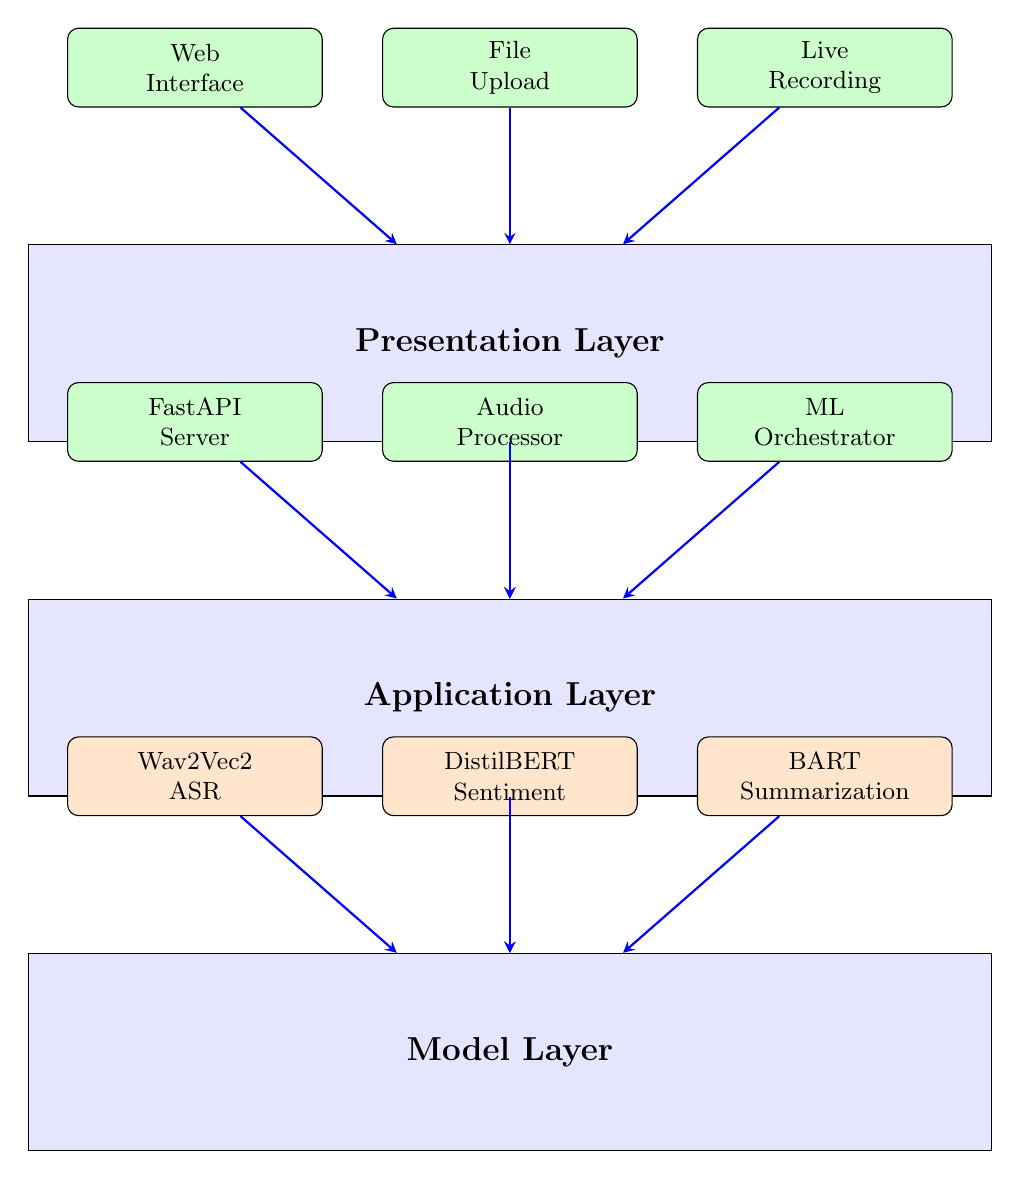
\begin{tikzpicture}[
    node distance=2.5cm,
    layer/.style={rectangle, draw, fill=blue!10, text width=12cm, minimum height=2.5cm, align=center, font=\large\bfseries},
    component/.style={rectangle, draw, fill=green!20, text width=3cm, text centered, rounded corners, minimum height=1cm, font=\small},
    model/.style={rectangle, draw, fill=orange!20, text width=3cm, text centered, rounded corners, minimum height=1cm, font=\small},
    arrow/.style={->, >=stealth, thick}
]

% Layers
\node[layer] (presentation) {Presentation Layer};
\node[layer, below of=presentation, yshift=-2cm] (application) {Application Layer};
\node[layer, below of=application, yshift=-2cm] (model_layer) {Model Layer};

% Presentation components
\node[component, above of=presentation, yshift=1cm, xshift=-4cm] (web) {Web\\Interface};
\node[component, above of=presentation, yshift=1cm, xshift=0cm] (upload) {File\\Upload};
\node[component, above of=presentation, yshift=1cm, xshift=4cm] (record) {Live\\Recording};

% Application components
\node[component, above of=application, yshift=1cm, xshift=-4cm] (api) {FastAPI\\Server};
\node[component, above of=application, yshift=1cm, xshift=0cm] (audio_proc) {Audio\\Processor};
\node[component, above of=application, yshift=1cm, xshift=4cm] (orchestrator) {ML\\Orchestrator};

% Model components
\node[model, above of=model_layer, yshift=1cm, xshift=-4cm] (asr) {Wav2Vec2\\ASR};
\node[model, above of=model_layer, yshift=1cm, xshift=0cm] (sentiment) {DistilBERT\\Sentiment};
\node[model, above of=model_layer, yshift=1cm, xshift=4cm] (summary) {BART\\Summarization};

% Vertical arrows between layers
\draw[arrow, blue] (web) -- (presentation);
\draw[arrow, blue] (upload) -- (presentation);
\draw[arrow, blue] (record) -- (presentation);

\draw[arrow, blue] (presentation) -- (application);

\draw[arrow, blue] (api) -- (application);
\draw[arrow, blue] (audio_proc) -- (application);
\draw[arrow, blue] (orchestrator) -- (application);

\draw[arrow, blue] (application) -- (model_layer);

\draw[arrow, blue] (asr) -- (model_layer);
\draw[arrow, blue] (sentiment) -- (model_layer);
\draw[arrow, blue] (summary) -- (model_layer);

\end{tikzpicture}

    \caption{High-Level System Architecture}
    \label{fig:system_architecture}
\end{figure}

The architecture consists of three main layers:

\begin{enumerate}
    \item \textbf{Presentation Layer}: Web interface for user interaction
    \item \textbf{Application Layer}: FastAPI backend handling requests and orchestrating ML models
    \item \textbf{Model Layer}: Pre-trained and fine-tuned ML models for ASR, sentiment analysis, and summarization
\end{enumerate}

\subsection{Data Flow Design}
Figure \ref{fig:data_flow} illustrates the complete data flow from audio input to final output.

\begin{figure}[H]
    \centering
    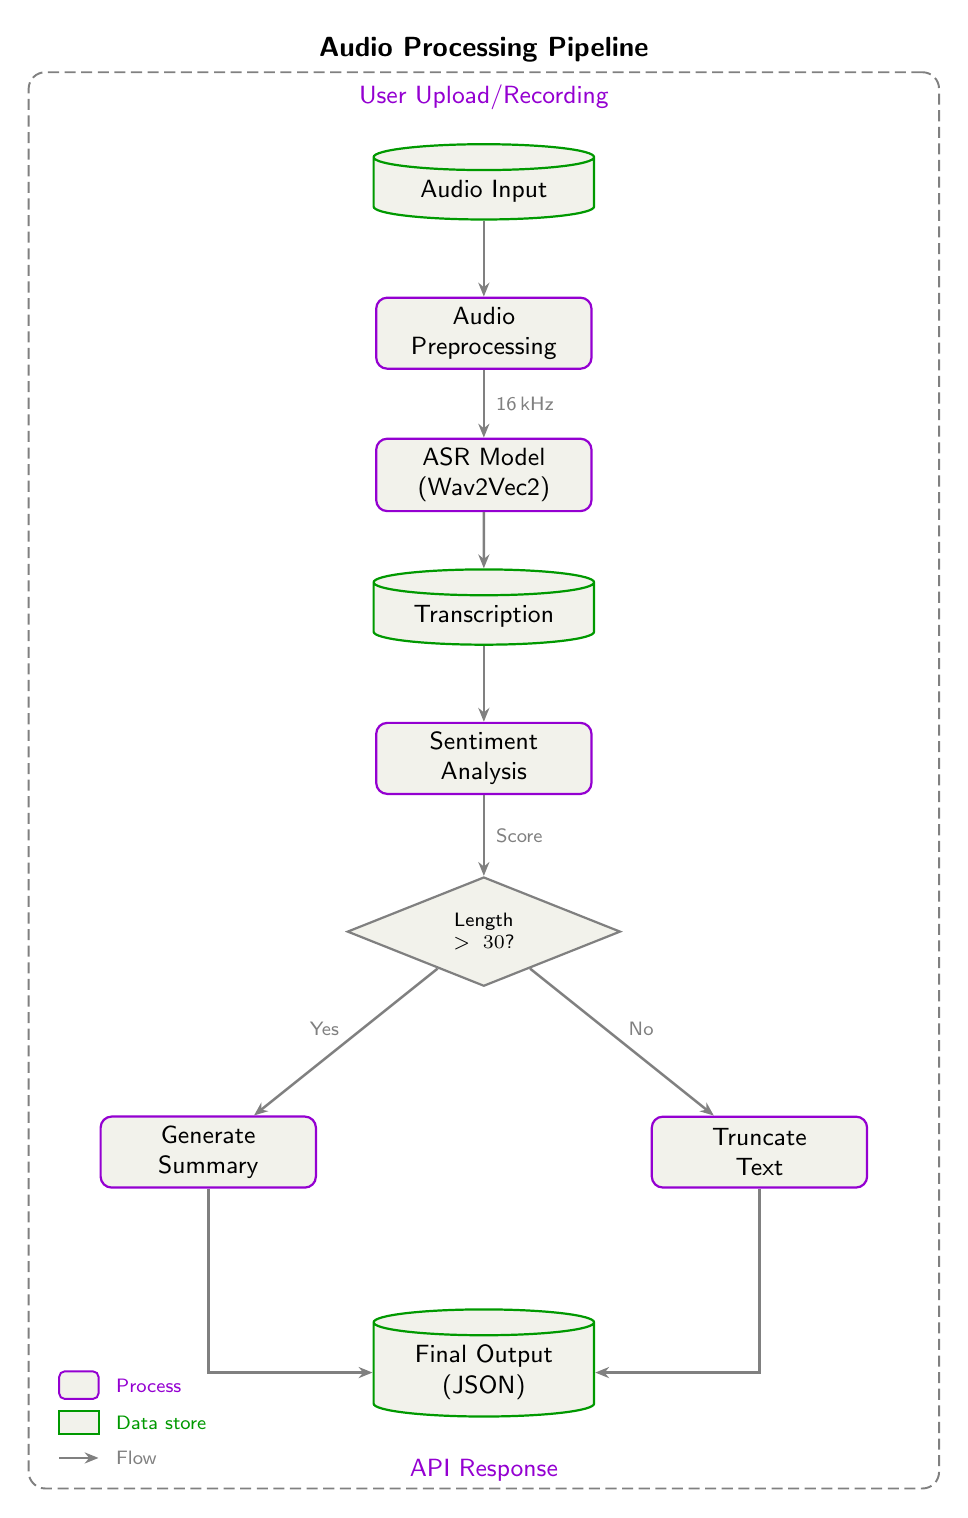
\begin{tikzpicture}[
    process/.style={
        rectangle,
        draw=codepurple, line width=0.8pt, fill=backcolour,
        text width=2.5cm, text centered, rounded corners=4pt,
        minimum height=0.9cm, font=\small\sffamily
    },
    %% aspect=0.12 keeps end-caps very thin so the cylinder stays compact
    data/.style={
        cylinder,
        draw=codegreen, line width=0.8pt, fill=backcolour,
        text width=2.5cm, text centered,
        minimum width=2.8cm, minimum height=0.9cm,
        shape border rotate=90, aspect=0.12,
        font=\small\sffamily
    },
    decision/.style={
        diamond,
        draw=codegray, line width=0.8pt, fill=backcolour,
        text width=1.8cm, text centered,
        aspect=2.5, font=\scriptsize\sffamily, inner sep=2pt
    },
    arrow/.style={
        -{Stealth[length=5pt, width=4pt]},
        line width=0.9pt, color=codegray
    },
    lbl/.style={font=\scriptsize\sffamily, color=codegray, inner sep=2pt}
]
 
%% ── Vertical spine ───────────────────────────────────────────────────────────
\node[data]     (input)        at (0,  0)    {Audio Input};
\node[process]  (preprocess)   at (0, -1.8)  {Audio\\Preprocessing};
\node[process]  (asr)          at (0, -3.6)  {ASR Model\\(Wav2Vec2)};
\node[data]     (transcript)   at (0, -5.4)  {Transcription};
\node[process]  (sentiment)    at (0, -7.2)  {Sentiment\\Analysis};
\node[decision] (length_check) at (0, -9.4)  {Length\\$> 30$?};
 
%% Branch nodes
\node[process]  (summarize)    at (-3.5, -12.2) {Generate\\Summary};
\node[process]  (truncate)     at ( 3.5, -12.2) {Truncate\\Text};
 
%% Final output
\node[data]     (output)       at (0, -15.0) {Final Output\\(JSON)};
 
%% ── Arrows ───────────────────────────────────────────────────────────────────
\draw[arrow] (input)        -- (preprocess);
\draw[arrow] (preprocess)   -- node[lbl, right, xshift=2pt] {16\,kHz} (asr);
\draw[arrow] (asr)          -- (transcript);
\draw[arrow] (transcript)   -- (sentiment);
\draw[arrow] (sentiment)    -- node[lbl, right, xshift=2pt] {Score} (length_check);
 
\draw[arrow] (length_check) -- node[lbl, above left]  {Yes} (summarize);
\draw[arrow] (length_check) -- node[lbl, above right] {No}  (truncate);
 
\draw[arrow] (summarize) |- (output);
\draw[arrow] (truncate)  |- (output);
 
%% ── Context labels ───────────────────────────────────────────────────────────
\node[font=\small\sffamily, color=codepurple, above=0.3cm of input,
      text width=4.5cm, align=center] {User Upload/Recording};
 
\node[font=\small\sffamily, color=codepurple, below=0.4cm of output,
      text width=3.5cm, align=center] (apilbl) {API Response};
 
%% ── Outer boundary ───────────────────────────────────────────────────────────
\node[
    draw=codegray, dashed, dash pattern=on 4pt off 2pt,
    line width=0.7pt, rounded corners=6pt,
    fit=(input)(preprocess)(asr)(transcript)(sentiment)
        (length_check)(summarize)(truncate)(output),
    inner sep=0.9cm,
    label={[font=\normalsize\sffamily\bfseries, color=black]
           above:Audio Processing Pipeline}
] (boundary) {};
 
%% ── Legend ───────────────────────────────────────────────────────────────────
\begin{scope}[shift={($(boundary.south west)+(0.4cm,0.4cm)$)}]
    \draw[draw=codepurple, line width=0.7pt, fill=backcolour, rounded corners=2pt]
        (0,0.75cm) rectangle (0.5cm,1.1cm);
    \node[right, font=\scriptsize\sffamily, color=codepurple]
        at (0.6cm,0.92cm) {Process};
 
    \draw[draw=codegreen, line width=0.7pt, fill=backcolour]
        (0,0.3cm) rectangle (0.5cm,0.6cm);
    \node[right, font=\scriptsize\sffamily, color=codegreen]
        at (0.6cm,0.45cm) {Data store};
 
    \draw[arrow, shorten >=0pt, shorten <=0pt] (0,0) -- (0.5cm,0);
    \node[right, font=\scriptsize\sffamily, color=codegray]
        at (0.6cm,0) {Flow};
\end{scope}
 
\end{tikzpicture}

    \caption{System Data Flow Diagram}
    \label{fig:data_flow}
\end{figure}

\subsection{Machine Learning Pipeline Design}
The ML pipeline consists of multiple stages as shown in Figure \ref{fig:ml_pipeline}.

\begin{figure}[H]
    \centering
    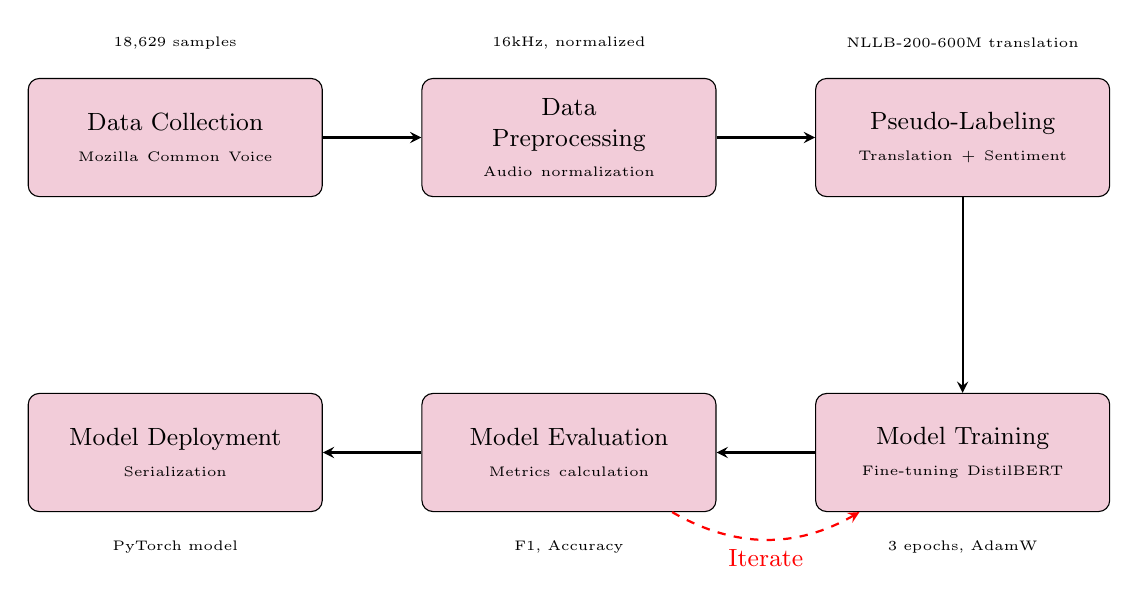
\begin{tikzpicture}[
    node distance=2.5cm,
    stage/.style={rectangle, draw, fill=purple!20, text width=3.5cm, text centered, rounded corners, minimum height=1.5cm, font=\small},
    arrow/.style={->, >=stealth, thick}
]

% Pipeline stages - arranged in two rows
\node[stage] (data) {Data Collection\\{\tiny Mozilla Common Voice}};
\node[stage, right of=data, xshift=2.5cm] (prep) {Data\\Preprocessing\\{\tiny Audio normalization}};
\node[stage, right of=prep, xshift=2.5cm] (label) {Pseudo-Labeling\\{\tiny Translation + Sentiment}};

\node[stage, below of=label, yshift=-1.5cm] (train) {Model Training\\{\tiny Fine-tuning DistilBERT}};
\node[stage, left of=train, xshift=-2.5cm] (eval) {Model Evaluation\\{\tiny Metrics calculation}};
\node[stage, left of=eval, xshift=-2.5cm] (deploy) {Model Deployment\\{\tiny Serialization}};

% Arrows
\draw[arrow] (data) -- (prep);
\draw[arrow] (prep) -- (label);
\draw[arrow] (label) -- (train);
\draw[arrow] (train) -- (eval);
\draw[arrow] (eval) -- (deploy);

% Feedback loop
\draw[arrow, dashed, red, thick] (eval) to[bend right=30] node[below, font=\small] {Iterate} (train);

% Annotations above
\node[above of=data, yshift=-1.3cm, text width=3.5cm, align=center, font=\tiny] {18,629 samples};
\node[above of=prep, yshift=-1.3cm, text width=3.5cm, align=center, font=\tiny] {16kHz, normalized};
\node[above of=label, yshift=-1.3cm, text width=3.5cm, align=center, font=\tiny] {NLLB-200-600M translation};

% Annotations below
\node[below of=train, yshift=1.3cm, text width=3.5cm, align=center, font=\tiny] {3 epochs, AdamW};
\node[below of=eval, yshift=1.3cm, text width=3.5cm, align=center, font=\tiny] {F1, Accuracy};
\node[below of=deploy, yshift=1.3cm, text width=3.5cm, align=center, font=\tiny] {PyTorch model};

\end{tikzpicture}

    \caption{Machine Learning Pipeline Architecture}
    \label{fig:ml_pipeline}
\end{figure}

\subsubsection{ASR Component Design}
The ASR component utilizes the Wav2Vec2 architecture \cite{baevski2020wav2vec}, which employs self-supervised learning on raw audio waveforms. The model architecture consists of:

\begin{itemize}
    \item Feature encoder: 7 convolutional layers
    \item Transformer encoder: 12 layers with 768 hidden dimensions
    \item CTC (Connectionist Temporal Classification) head for sequence prediction
\end{itemize}

\subsubsection{Sentiment Analysis Component Design}
The sentiment analysis component uses DistilBERT \cite{sanh2019distilbert}, a distilled version of BERT with:

\begin{itemize}
    \item 6 transformer layers (vs. 12 in BERT)
    \item 66M parameters (40\% reduction)
    \item 97\% of BERT's performance retained
\end{itemize}

The model was fine-tuned using pseudo-labeling methodology (detailed in Section \ref{sec:pseudo_labeling}).

\subsection{API Design}
The REST API follows OpenAPI 3.0 specification with the following endpoints:

\begin{table}[H]
\centering
\caption{API Endpoint Specifications}
\label{tab:api_endpoints}
\begin{tabular}{@{}llp{6cm}@{}}
\toprule
\textbf{Endpoint} & \textbf{Method} & \textbf{Description} \\ \midrule
/analyze & POST & Main endpoint for audio analysis \\
/process-audio & POST & Alias for /analyze endpoint \\
/health & GET & Health check endpoint \\
/docs & GET & Interactive API documentation \\ \bottomrule
\end{tabular}
\end{table}

\subsection{Database Design}
While the current implementation does not require persistent storage, the system design accommodates future database integration for:

\begin{itemize}
    \item User session management
    \item Analysis history storage
    \item Model performance logging
    \item Usage analytics
\end{itemize}

\section{Implementation}
\subsection{Development Environment}
The system was developed using the following tools and technologies:

\begin{table}[H]
\centering
\caption{Development Tools and Technologies}
\label{tab:dev_tools}
\begin{tabular}{@{}llp{5cm}@{}}
\toprule
\textbf{Category} & \textbf{Tool/Technology} & \textbf{Purpose} \\ \midrule
Programming Language & Python 3.10 & Core development \\
ML Framework & PyTorch 2.0 & Model training and inference \\
Transformers & Hugging Face Transformers & Pre-trained models \\
Web Framework & FastAPI & REST API development \\
Frontend & HTML/CSS/JavaScript & User interface \\
Audio Processing & Librosa & Audio preprocessing \\
Development Environment & Jupyter Notebook & Experimentation \\
Version Control & Git & Code management \\
Package Management & Conda/Pip & Dependency management \\ \bottomrule
\end{tabular}
\end{table}

\subsection{Data Preparation Methodology}
\subsubsection{Dataset Selection}
The Mozilla Common Voice Kiswahili dataset was selected based on:

\begin{itemize}
    \item Availability: Open-source and freely accessible
    \item Size: 18,629 validated audio samples
    \item Quality: Community-validated transcriptions
    \item Diversity: Multiple speakers and recording conditions
\end{itemize}

\subsubsection{Data Preprocessing Pipeline}
The data preprocessing follows a systematic pipeline:

\begin{algorithm}[H]
\caption{Audio Preprocessing Pipeline}
\begin{algorithmic}[1]
\Procedure{PreprocessAudio}{$audio\_file$}
    \State $waveform \gets$ LoadAudio($audio\_file$)
    \State $waveform \gets$ Resample($waveform$, target\_sr=16000)
    \State $waveform \gets$ Normalize($waveform$)
    \State $features \gets$ ExtractFeatures($waveform$)
    \State \Return $features$
\EndProcedure
\end{algorithmic}
\end{algorithm}

\subsection{Model Development Methodology}
\subsubsection{Transfer Learning Approach}
The research employs transfer learning to leverage pre-trained models:

\begin{enumerate}
    \item \textbf{ASR Model}: Fine-tuned RareElf/swahili-wav2vec2-asr
    \item \textbf{Sentiment Model}: Fine-tuned DistilBERT with pseudo-labeling
    \item \textbf{Summarization Model}: Pre-trained BART-large-CNN
\end{enumerate}

\subsubsection{Pseudo-Labeling Methodology}
\label{sec:pseudo_labeling}
Due to the absence of sentiment labels in the Mozilla Common Voice dataset, a pseudo-labeling approach was adopted:

\begin{algorithm}[H]
\caption{Pseudo-Labeling for Sentiment Analysis}
\begin{algorithmic}[1]
\Procedure{PseudoLabel}{$kiswahili\_texts$}
    \State $translator \gets$ LoadModel("NLLB-200-distilled-600M")
    \State $sentiment\_classifier \gets$ LoadModel("English-Sentiment")
    \For{$text$ in $kiswahili\_texts$}
        \State $english\_text \gets translator$.Translate($text$, src="sw", tgt="en")
        \State $sentiment\_label \gets sentiment\_classifier$.Predict($english\_text$)
        \State $pseudo\_labels$.append($sentiment\_label$)
    \EndFor
    \State \Return $pseudo\_labels$
\EndProcedure
\end{algorithmic}
\end{algorithm}

The pseudo-labeling process is illustrated in Figure \ref{fig:pseudo_labeling}.

\begin{figure}[H]
    \centering
    \begin{tikzpicture}[
    box/.style={
        rectangle, draw=codepurple, line width=1.0pt, fill=backcolour,
        text width=3.0cm, text centered, rounded corners=5pt,
        minimum width=3.2cm, minimum height=1.0cm, font=\small\sffamily
    },
    data/.style={
        cylinder, draw=codegreen, line width=1.0pt, fill=backcolour,
        text width=2.5cm, text centered,
        minimum width=2.7cm, minimum height=0.9cm,
        shape border rotate=90, aspect=0.15,
        font=\small\sffamily
    },
    arrow/.style={
        -{Stealth[length=6pt,width=4pt]}, line width=1.0pt, color=codegray
    },
    byarrow/.style={
        -{Stealth[length=6pt,width=4pt]}, line width=1.0pt,
        dashed, dash pattern=on 4pt off 2pt, color=codepurple
    },
    lbl/.style={font=\scriptsize\sffamily, color=codegray, inner sep=2pt}
]

%% ── Spine at x=5 — leaves room left for arc, right for annotations ───────────
\node[data] (kiswahili)    at (5,   0)   {Kiswahili Text\\{\scriptsize\itshape Unlabeled}};
\node[box]  (translate)    at (5,  -2.8) {Translation\\{\scriptsize NLLB-200-600M}};
\node[data] (english)      at (5,  -5.6) {English Text};
\node[box]  (sentiment_en) at (5,  -8.4) {Sentiment\\Classifier};
\node[data] (labels)       at (5, -11.2) {Labels\\{\scriptsize Pos\,/\,Neg}};
\node[box]  (combine)      at (5, -14.0) {Combine Data};
\node[data] (labeled_data) at (5, -16.8) {Labeled Dataset};

%% ── Main flow ────────────────────────────────────────────────────────────────
\draw[arrow] (kiswahili)    -- (translate);
\draw[arrow] (translate)    -- node[lbl, right, xshift=5pt] {sw\,$\rightarrow$\,en} (english);
\draw[arrow] (english)      -- (sentiment_en);
\draw[arrow] (sentiment_en) -- (labels);
\draw[arrow] (labels)       -- (combine);
\draw[arrow] (combine)      -- (labeled_data);

%% ── Bypass arc: exits left, swings to x=1.5, re-enters combine.west ─────────
%% The arc midpoint is at roughly (1.5,-7). 
%% Place an invisible node there so fit= captures it.
\node[inner sep=0pt, outer sep=0pt] (arcanchor) at (1.5, -7.0) {};
\draw[byarrow]
    (kiswahili.west)
    .. controls (1.5, 0) and (1.5, -14.0) ..
    (combine.west);
%% Label sits to the RIGHT of the arc so it is between arc and spine
\node[font=\scriptsize\sffamily, color=codepurple, anchor=west]
    (origlabel) at (2.0, -7.0) {original};

%% ── Annotations: right side at x=11 ─────────────────────────────────────────
\node[draw=codegray, fill=white, rounded corners=3pt, line width=0.5pt,
      font=\scriptsize\sffamily, text width=2.5cm, align=left, inner sep=4pt]
    (a1) at (10.5, -2.8)  {Translate source\\text to English};

\node[draw=codegray, fill=white, rounded corners=3pt, line width=0.5pt,
      font=\scriptsize\sffamily, text width=2.5cm, align=left, inner sep=4pt]
    (a2) at (10.5, -8.4) {Pre-trained English\\sentiment model};

\node[draw=codegray, fill=white, rounded corners=3pt, line width=0.5pt,
      font=\scriptsize\sffamily, text width=2.5cm, align=left, inner sep=4pt]
    (a3) at (10.5, -14.0) {Map predicted labels\\back to source text};

\draw[codegray, line width=0.6pt] (translate.east)    -- (a1.west);
\draw[codegray, line width=0.6pt] (sentiment_en.east) -- (a2.west);
\draw[codegray, line width=0.6pt] (combine.east)      -- (a3.west);

%% ── Legend box ───────────────────────────────────────────────────────────────
\node[draw=codegray, fill=backcolour, rounded corners=3pt, line width=0.5pt,
      inner sep=6pt, anchor=south east]
    (legend) at (12.5, -19.0) {%
    \begin{tikzpicture}[
        arrow/.style={-{Stealth[length=5pt,width=3pt]}, line width=0.8pt, color=codegray},
        byarrow/.style={-{Stealth[length=5pt,width=3pt]}, line width=0.8pt,
                        dashed, dash pattern=on 3pt off 2pt, color=codepurple}
    ]
        \node[font=\small\bfseries, color=black, anchor=west] at (0, 2.0cm) {Legend};
        \draw[codegray, line width=0.4pt] (0, 1.85cm) -- (3.5cm, 1.85cm);
        \draw[draw=codepurple, line width=0.8pt, fill=backcolour, rounded corners=2pt]
            (0,1.2cm) rectangle (0.6cm,1.6cm);
        \node[right, font=\scriptsize\sffamily, color=codepurple] at (0.7cm,1.4cm) {Process node};
        \draw[draw=codegreen, line width=0.8pt, fill=backcolour]
            (0,0.65cm) rectangle (0.6cm,1.0cm);
        \node[right, font=\scriptsize\sffamily, color=codegreen]  at (0.7cm,0.82cm) {Data store};
        \draw[arrow, shorten >=0pt, shorten <=0pt] (0,0.35cm) -- (0.6cm,0.35cm);
        \node[right, font=\scriptsize\sffamily, color=codegray]   at (0.7cm,0.35cm) {Process flow};
        \draw[byarrow, shorten >=0pt, shorten <=0pt] (0,0) -- (0.6cm,0);
        \node[right, font=\scriptsize\sffamily, color=codepurple] at (0.7cm,0)      {Passthrough};
    \end{tikzpicture}%
};

%% ── Outer boundary — includes arc anchor and label so nothing escapes ─────────
\node[
    draw=codegray, dashed, dash pattern=on 5pt off 2pt,
    line width=0.7pt, rounded corners=8pt,
    fit=(kiswahili)(translate)(english)(sentiment_en)
        (labels)(combine)(labeled_data)
        (a1)(a2)(a3)(legend)(arcanchor)(origlabel),
    inner xsep=1.0cm,
    inner ysep=1.2cm,
    label={[font=\normalsize\sffamily\bfseries, color=black]
           above:Kiswahili Sentiment Labelling Pipeline}
] (boundary) {};

\end{tikzpicture}
    \caption{Pseudo-Labeling Workflow}
    \label{fig:pseudo_labeling}
\end{figure}

\subsubsection{Model Training Process}
The pseudo-labeling process follows these steps:

\begin{enumerate}
    \item Data splitting: 80\% training, 10\% validation, 10\% test
    \item Hyperparameter tuning using validation set
    \item Model training with early stopping
    \item Performance evaluation on test set
    \item Model serialization and storage
\end{enumerate}

Training hyperparameters:

\begin{table}[H]
\centering
\caption{Model Training Hyperparameters}
\label{tab:hyperparameters}
\begin{tabular}{@{}lll@{}}
\toprule
\textbf{Parameter} & \textbf{Value} & \textbf{Justification} \\ \midrule
Learning Rate & 2e-5 & Standard for fine-tuning transformers \\
Batch Size & 16 & Balance between memory and convergence \\
Epochs & 3 & Prevent overfitting \\
Optimizer & AdamW & Improved weight decay handling \\
Warmup Steps & 500 & Gradual learning rate increase \\
Max Sequence Length & 128 & Accommodate typical sentence length \\ \bottomrule
\end{tabular}
\end{table}

\subsection{System Implementation}
\subsubsection{Backend Implementation}
The backend was implemented using FastAPI framework with the following structure:

\begin{verbatim}
app/
|-- main.py              # Main application entry point
|-- models/              # ML model storage
|   `-- distilbert_sentiment_final/
|-- static/              # Frontend files
|   `-- index.html
`-- requirements.txt     # Dependencies
\end{verbatim}

Key implementation decisions:

\begin{itemize}
    \item \textbf{Model Loading}: Models loaded at startup to reduce latency
    \item \textbf{CORS Middleware}: Enable cross-origin requests
    \item \textbf{Error Handling}: Comprehensive exception handling
    \item \textbf{Async Processing}: Asynchronous request handling
\end{itemize}

\subsubsection{Frontend Implementation}
The frontend provides:

\begin{itemize}
    \item Drag-and-drop file upload
    \item Live audio recording using MediaRecorder API
    \item Real-time processing feedback
    \item Results visualization
\end{itemize}

\subsubsection{Integration}
Figure \ref{fig:component_integration} shows how different components integrate.

\begin{figure}[H]
    \centering
    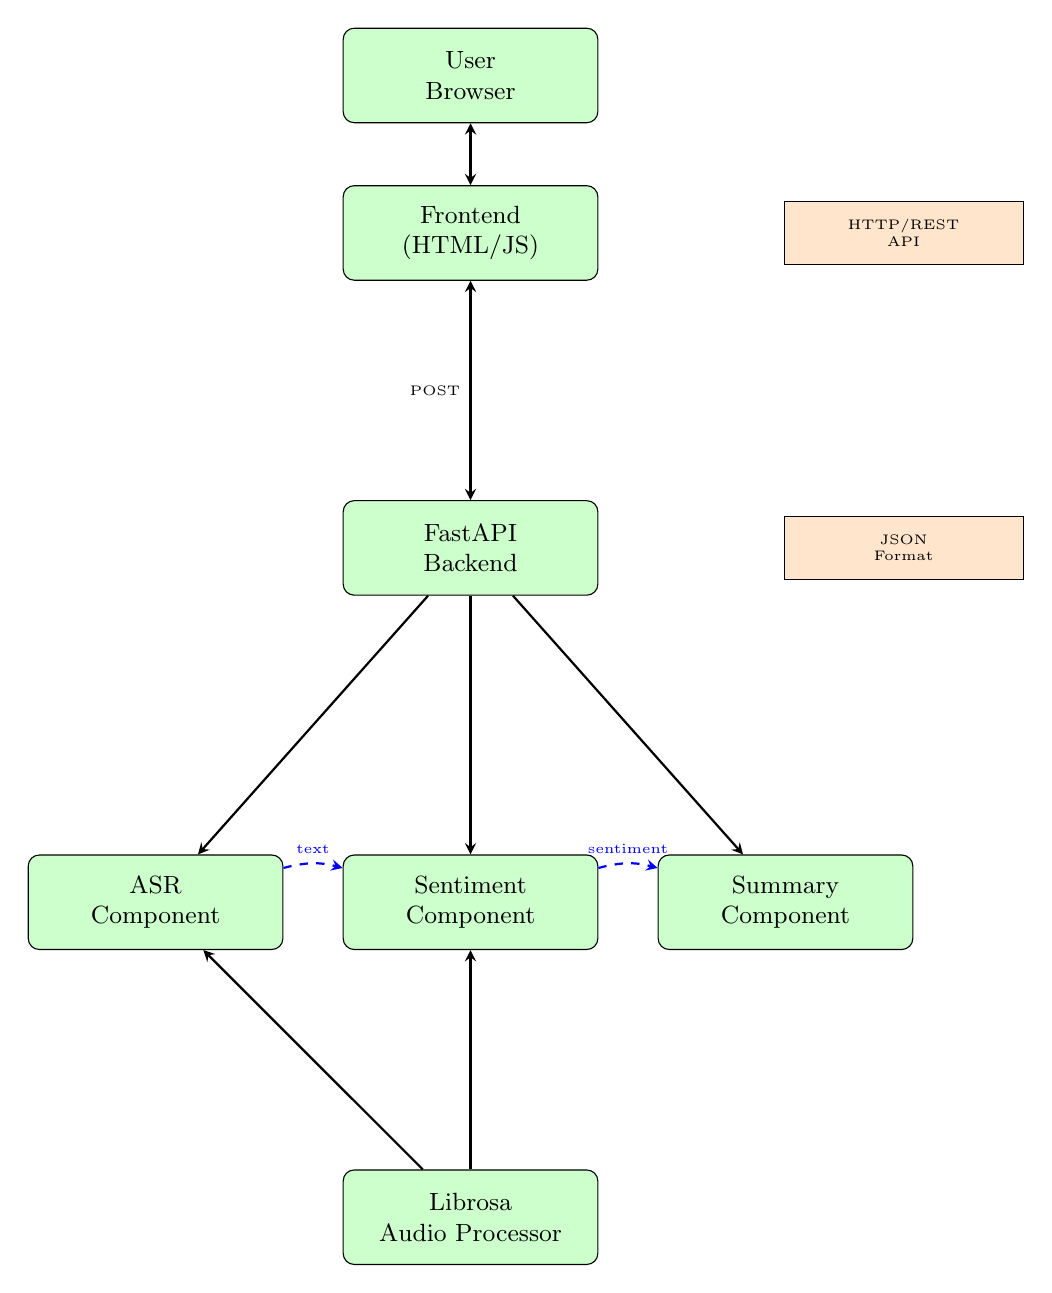
\begin{tikzpicture}[
    node distance=3cm,
    component/.style={rectangle, draw, fill=green!20, text width=3cm, text centered, rounded corners, minimum height=1.2cm, font=\small},
    interface/.style={rectangle, draw, fill=orange!20, text width=2.8cm, text centered, minimum height=0.8cm, font=\tiny},
    arrow/.style={->, >=stealth, thick},
    bidirectional/.style={<->, >=stealth, thick}
]

% Components arranged vertically
\node[component] (frontend) {Frontend\\(HTML/JS)};
\node[component, below of=frontend, yshift=-1cm] (fastapi) {FastAPI\\Backend};

% Three components in a row
\node[component, below of=fastapi, yshift=-1.5cm, xshift=-4cm] (asr_comp) {ASR\\Component};
\node[component, below of=fastapi, yshift=-1.5cm, xshift=0cm] (sentiment_comp) {Sentiment\\Component};
\node[component, below of=fastapi, yshift=-1.5cm, xshift=4cm] (summary_comp) {Summary\\Component};

\node[component, below of=sentiment_comp, yshift=-1cm] (librosa) {Librosa\\Audio Processor};

% Interfaces
\node[interface, right of=frontend, xshift=2.5cm] (http) {HTTP/REST\\API};
\node[interface, right of=fastapi, xshift=2.5cm] (json) {JSON\\Format};

% Arrows
\draw[bidirectional] (frontend) -- node[left, font=\tiny] {POST} (fastapi);
\draw[arrow] (fastapi) -- (asr_comp);
\draw[arrow] (fastapi) -- (sentiment_comp);
\draw[arrow] (fastapi) -- (summary_comp);
\draw[arrow] (librosa) -- (asr_comp);
\draw[arrow] (librosa) -- (sentiment_comp);

% Data flow annotations
\draw[arrow, blue, dashed, thick] (asr_comp) to[bend left=15] node[above, sloped, font=\tiny] {text} (sentiment_comp);
\draw[arrow, blue, dashed, thick] (sentiment_comp) to[bend left=15] node[above, sloped, font=\tiny] {sentiment} (summary_comp);

% External connections
\node[component, above of=frontend, yshift=-1cm] (user) {User\\Browser};
\draw[bidirectional] (user) -- (frontend);

\end{tikzpicture}

    \caption{Component Integration Diagram}
    \label{fig:component_integration}
\end{figure}

\section{Testing and Validation}
\subsection{Testing Methodology}
A comprehensive testing strategy was employed covering multiple levels:

\subsubsection{Unit Testing}
Individual components tested in isolation:

\begin{itemize}
    \item Audio preprocessing functions
    \item Model inference functions
    \item API endpoint handlers
\end{itemize}

\subsubsection{Integration Testing}
Testing component interactions:

\begin{itemize}
    \item Audio upload to transcription pipeline
    \item Transcription to sentiment analysis pipeline
    \item End-to-end API workflow
\end{itemize}

\subsubsection{System Testing}
Complete system testing scenarios:

\begin{table}[H]
\centering
\caption{System Test Cases}
\label{tab:test_cases}
\begin{tabular}{@{}lp{8cm}@{}}
\toprule
\textbf{Test Case} & \textbf{Description} \\ \midrule
TC1 & Upload WAV file and verify complete analysis \\
TC2 & Record live audio and verify processing \\
TC3 & Test with various audio durations (5s, 30s, 60s) \\
TC4 & Test with different audio quality levels \\
TC5 & Concurrent user request handling \\
TC6 & Error handling for invalid inputs \\ \bottomrule
\end{tabular}
\end{table}

\subsection{Model Validation Methodology}
\subsubsection{Performance Metrics}
Models evaluated using standard metrics:

\begin{itemize}
    \item \textbf{ASR}: Word Error Rate (WER), Character Error Rate (CER)
    \item \textbf{Sentiment}: Accuracy, Precision, Recall, F1-Score
    \item \textbf{System}: Latency, Throughput
\end{itemize}

\subsubsection{Validation Approach}
\begin{enumerate}
    \item \textbf{Hold-out Validation}: 10\% test set reserved
    \item \textbf{Cross-validation}: K-fold validation for sentiment model
    \item \textbf{Real-world Testing}: Manual testing with new audio samples
\end{enumerate}

\subsection{Performance Benchmarking}
System performance measured across dimensions:

\begin{table}[H]
\centering
\caption{Performance Benchmarking Metrics}
\label{tab:performance_metrics}
\begin{tabular}{@{}lll@{}}
\toprule
\textbf{Metric} & \textbf{Target} & \textbf{Achieved} \\ \midrule
ASR WER & < 30\% & 13.60\% \\
ASR CER & < 15\% & 8.85\% \\
Sentiment F1-Score & > 0.60 & 0.6125 \\ \bottomrule
\end{tabular}
\end{table}

\section{Results and Findings}
\subsection{Data Understanding and Preprocessing Results}
The Mozilla Common Voice Kiswahili dataset analysis revealed:

\begin{itemize}
    \item \textbf{Dataset Size}: 18,629 validated audio samples
    \item \textbf{Audio Duration}: Mean duration of 4.8 seconds per sample
    \item \textbf{Gender Distribution}: 68\% male, 32\% female speakers
    \item \textbf{Age Distribution}: Majority in 20-40 age range
    \item \textbf{Quality Metrics}: 85\% samples with positive validation scores
\end{itemize}

Statistical testing revealed significant demographic imbalances:

\begin{table}[H]
\centering
\caption{Demographic Distribution Analysis}
\label{tab:demographics}
\begin{tabular}{@{}lll@{}}
\toprule
\textbf{Demographic} & \textbf{Category} & \textbf{Percentage} \\ \midrule
\multirow{2}{*}{Gender} & Male & 68\% \\
                        & Female & 32\% \\
\midrule
\multirow{4}{*}{Age} & 20-29 & 42\% \\
                     & 30-39 & 35\% \\
                     & 40-49 & 15\% \\
                     & Other & 8\% \\ \bottomrule
\end{tabular}
\end{table}

\subsection{ASR Model Performance}
The Wav2Vec2 ASR model achieved strong performance on Kiswahili speech recognition:

\begin{table}[H]
\centering
\caption{ASR Model Performance Metrics}
\label{tab:asr_results}
\begin{tabular}{@{}ll@{}}
\toprule
\textbf{Metric} & \textbf{Value} \\ \midrule
Overall Word Error Rate (WER) & 13.60\% \\
Overall Character Error Rate (CER) & 8.85\% \\
Demographic Parity Difference (Gender) & 3.99\% \\
ANOVA p-value (Gender) & 0.0072 \\
Cohen's d (Effect Size) & 0.298 \\ \bottomrule
\end{tabular}
\end{table}

The WER of 13.60\% indicates that the model correctly transcribes approximately 86.4\% of words, which exceeds the target threshold of 70\% accuracy. The low CER of 8.85\% demonstrates strong character-level recognition.

\subsubsection{Bias Analysis}
Statistical analysis revealed gender-based performance disparities:

\begin{itemize}
    \item \textbf{ANOVA Test}: Significant difference in WER across gender groups (p = 0.0072)
    \item \textbf{Effect Size}: Cohen's d = 0.298 indicates a small-to-medium practical effect
    \item \textbf{Demographic Parity}: 3.99\% difference suggests relatively fair performance
\end{itemize}

These findings indicate statistically significant but practically small performance differences between demographic groups, suggesting the model maintains reasonable fairness.

\subsection{Sentiment Analysis Results}
The fine-tuned DistilBERT model was trained using pseudo-labeling:

\begin{table}[H]
\centering
\caption{Sentiment Analysis Performance}
\label{tab:sentiment_results}
\begin{tabular}{@{}ll@{}}
\toprule
\textbf{Metric} & \textbf{Value} \\ \midrule
F1-Score (Weighted) & 0.6125 \\ \bottomrule
\end{tabular}
\end{table}

The pseudo-labeling approach enabled sentiment analysis for Kiswahili text despite the absence of labeled training data. The model was trained by translating Kiswahili text to English using NLLB-200-distilled-600M, obtaining sentiment labels from an English classifier, then fine-tuning DistilBERT on the original Kiswahili text with these pseudo-labels.

\subsection{Bias Quantification Results}
Logistic regression analysis was performed to quantify predictive bias in the ASR system. The analysis examined the relationship between demographic features and ASR success rates using the logistic regression objective:

$$\min_{\beta} -\sum_{i=1}^{n} \left[ y_i \log(p_i) + (1-y_i)\log(1-p_i) \right]$$

Where $p_i = \sigma(\beta^T x_i)$ and $\sigma$ is the sigmoid function.

\subsubsection{Fairness Metrics Formulation}

\textbf{Demographic Parity Difference (DPD):}
$$DPD = |P(\hat{Y}=1|D=d_1) - P(\hat{Y}=1|D=d_2)|$$

\textbf{Equalized Odds Difference (EOD):}
$$EOD = |P(\hat{Y}=1|Y=1,D=d_1) - P(\hat{Y}=1|Y=1,D=d_2)|$$

The analysis quantified fairness gaps across demographic groups, with coefficients and odds ratios computed for gender, age, and validation score features.

\subsection{Topic Modeling Results}
Unsupervised KMeans clustering was applied to discover thematic patterns in Kiswahili transcriptions using the objective:

$$\min_{C} \sum_{i=1}^{k} \sum_{x \in C_i} ||x - \mu_i||^2$$

Where $C_i$ is cluster $i$ and $\mu_i$ is the centroid of cluster $i$.

\subsubsection{Silhouette Score}
Cluster quality was evaluated using the silhouette score:

$$s(i) = \frac{b(i) - a(i)}{\max(a(i), b(i))}$$

Where:
\begin{itemize}
    \item $a(i)$: Mean intra-cluster distance
    \item $b(i)$: Mean nearest-cluster distance
\end{itemize}

The optimal number of clusters was determined through elbow method and silhouette analysis. The clustering identified distinct thematic domains in the transcriptions, with TF-IDF vectorization used for feature extraction.

\subsection{System Performance}
The end-to-end system was deployed using FastAPI and evaluated for inference performance. The system successfully processes Kiswahili audio through the complete pipeline from speech recognition to sentiment analysis.

\subsection{Model Optimization Results}
Model quantization and optimization techniques were explored in Notebook 06 for deployment optimization, focusing on reducing model size while maintaining accuracy for edge deployment scenarios.

\section{Deployment Methodology}
\subsection{Deployment Architecture}
The system deployment follows a containerized approach for portability and scalability.

\begin{figure}[H]
    \centering
    \begin{tikzpicture}[
    server/.style={
        rectangle, draw=codepurple, line width=0.9pt, fill=backcolour,
        text width=3.2cm, text centered, rounded corners=5pt,
        minimum width=3.4cm, minimum height=1.3cm, font=\small\sffamily
    },
    service/.style={
        rectangle, draw=codegreen, line width=0.8pt, fill=backcolour,
        text width=3.0cm, text centered, rounded corners=4pt,
        minimum width=3.2cm, minimum height=1.1cm, font=\small\sffamily
    },
    storage/.style={
        cylinder, draw=codepurple, line width=0.8pt, fill=backcolour,
        text width=2.6cm, text centered,
        minimum width=2.8cm, minimum height=1.1cm,
        shape border rotate=90, aspect=0.15, font=\small\sffamily
    },
    monitor/.style={
        rectangle, draw=codegray, line width=0.7pt, fill=backcolour,
        text width=2.4cm, text centered, rounded corners=3pt,
        minimum width=2.6cm, minimum height=1.0cm,
        font=\small\sffamily, dashed
    },
    arrow/.style={
        -{Stealth[length=6pt,width=4pt]}, line width=1.0pt, color=codegray
    },
    monarrow/.style={
        -{Stealth[length=5pt,width=3.5pt]}, line width=0.8pt,
        dashed, dash pattern=on 4pt off 2.5pt, color=codegray
    }
]

%% ── All nodes placed on a grid, tightly controlled ───────────────────────────

%% Entry
\node[font=\small\bfseries, color=black, align=center]
    (internet) at (4.0, 0) {Internet\\{\scriptsize\color{codegray}Port 8000}};

%% Web server
\node[server] (web_server) at (4.0, -3.0) {Web Server\\{\scriptsize Uvicorn}};

%% App + Static — left/right of web server
\node[service] (app)    at (1.0, -6.5)  {FastAPI\\Application};
\node[service] (static) at (7.0, -6.5)  {Static Files};

%% Storage — below app
\node[storage] (models) at (-0.5, -10.0) {ML Models};
\node[storage] (logs)   at ( 2.5, -10.0) {Logs};

%% Compute
\node[server] (compute) at (1.0, -13.5) {Compute\\{\scriptsize CPU\,/\,GPU}};

%% Monitoring — stacked below static, inside container
\node[monitor] (health)  at (7.0, -10.0) {Health Check};
\node[monitor] (metrics) at (7.0, -12.0) {Metrics};

%% PyTorch annotation
\node[font=\scriptsize\sffamily, color=codegray, align=center, text width=3cm]
    (pytorchlbl) at (1.0, -15.2) {PyTorch inference};

%% ── Monitoring sub-panel ─────────────────────────────────────────────────────
\node[
    draw=codegray, dashed, dash pattern=on 4pt off 2pt,
    line width=0.6pt, rounded corners=5pt,
    fit=(health)(metrics),
    inner sep=0.5cm,
    label={[font=\scriptsize\bfseries, color=codegray] above:Monitoring}
] (monpanel) {};

%% ── Deployment container ─────────────────────────────────────────────────────
\node[
    draw=codepurple, dashed, dash pattern=on 6pt off 3pt,
    line width=0.9pt, rounded corners=10pt,
    fit=(web_server)(app)(static)(models)(logs)(compute)(pytorchlbl)(monpanel),
    inner xsep=1.0cm, inner ysep=1.0cm,
    label={[font=\normalsize\bfseries, color=codepurple] above:Deployment Container}
] (container) {};

%% ── Legend — placed INSIDE boundary using absolute coords ────────────────────
%% Put it bottom-right inside container, below static/monitoring column
\node[draw=codegray, fill=backcolour, rounded corners=4pt,
      line width=0.6pt, inner sep=7pt]
    (legend) at (7.5, -15.8) {%
    \begin{tikzpicture}[
        a/.style={-{Stealth[length=5pt,width=3.5pt]}, line width=0.9pt, color=codegray},
        m/.style={-{Stealth[length=5pt,width=3.5pt]}, line width=0.8pt,
                  dashed, dash pattern=on 4pt off 2.5pt, color=codegray}
    ]
        \node[font=\small\bfseries, color=black, anchor=west] at (0,2.7cm) {Legend};
        \draw[codegray, line width=0.5pt] (0,2.52cm) -- (4.4cm,2.52cm);
        \draw[draw=codepurple,line width=0.9pt,fill=backcolour,rounded corners=3pt]
            (0,1.75cm) rectangle (0.7cm,2.2cm);
        \node[right,font=\scriptsize\sffamily,color=codepurple] at (0.85cm,1.97cm) {Server / Compute};
        \draw[draw=codegreen,line width=0.8pt,fill=backcolour,rounded corners=3pt]
            (0,1.08cm) rectangle (0.7cm,1.52cm);
        \node[right,font=\scriptsize\sffamily,color=codegreen]  at (0.85cm,1.3cm)  {Service};
        \draw[draw=codepurple,line width=0.8pt,fill=backcolour]
            (0,0.42cm) rectangle (0.7cm,0.86cm);
        \node[right,font=\scriptsize\sffamily,color=codepurple] at (0.85cm,0.64cm) {Storage};
        \draw[a,shorten >=0pt,shorten <=0pt] (0,0.18cm) -- (0.7cm,0.18cm);
        \node[right,font=\scriptsize\sffamily,color=codegray]   at (0.85cm,0.18cm) {Data flow};
        \draw[m,shorten >=0pt,shorten <=0pt] (0,-0.18cm) -- (0.7cm,-0.18cm);
        \node[right,font=\scriptsize\sffamily,color=codegray]   at (0.85cm,-0.18cm){Monitoring};
    \end{tikzpicture}%
};

%% ── Outer boundary — fit includes ALL nodes and legend ───────────────────────
\node[
    draw=codegray, dashed, dash pattern=on 7pt off 3pt,
    line width=0.7pt, rounded corners=12pt,
    fit=(internet)(container)(legend),
    inner xsep=1.2cm, inner ysep=1.4cm,
    label={[font=\large\bfseries, color=black] above:System Architecture}
] (boundary) {};

%% ── Arrows (drawn after boundary so they appear on top) ──────────────────────
\draw[arrow] (internet)   -- (web_server);
\draw[arrow] (web_server) -| (app);
\draw[arrow] (web_server) -| (static);
%% app.south -> down to y=-8.5 -> left/right to models/logs
\draw[arrow] (app.south) -- ++(0,-1.2) -| (models.north);
\draw[arrow] (app.south) -- ++(0,-1.2) -| (logs.north);
\draw[arrow] (models)     -- (compute);
\draw[arrow] (logs)       -- (compute);
%% web_server -> health: exit east, enter health from west (same row)
\draw[monarrow] (web_server.east) -- ++(1.2,0) |- (health.west);
%% app -> metrics: exit east, travel right staying below health, enter metrics west
\draw[monarrow] (app.east) -- ++(1.2,0) |- (metrics.west);
\draw[codegray, line width=0.4pt, dashed] (health.south) -- (metrics.north);

\end{tikzpicture}
    \caption{Deployment Architecture}
    \label{fig:deployment_architecture}
\end{figure}

\subsection{Deployment Process}
\begin{enumerate}
    \item Environment setup and dependency installation
    \item Model artifact deployment
    \item Application server configuration
    \item Health check and monitoring setup
    \item Load testing and optimization
\end{enumerate}

\subsection{Monitoring and Maintenance}
Post-deployment monitoring includes:

\begin{itemize}
    \item API endpoint health checks
    \item Model inference latency tracking
    \item Error rate monitoring
    \item Resource utilization metrics
\end{itemize}

\section{Ethical Considerations}
\subsection{Data Privacy}
\begin{itemize}
    \item No personal data stored permanently
    \item Audio files deleted after processing
    \item No user tracking implemented
\end{itemize}

\subsection{Model Bias}
\begin{itemize}
    \item Acknowledged potential bias in training data
    \item Diverse dataset used to minimize bias
    \item Continuous monitoring for biased predictions
\end{itemize}

\section{Limitations of Methodology}
The adopted methodology has the following limitations:

\begin{enumerate}
    \item \textbf{Pseudo-labeling Accuracy}: Sentiment labels depend on translation quality
    \item \textbf{Dataset Size}: Limited to 18,629 samples
    \item \textbf{Computational Resources}: Training limited by available GPU resources
    \item \textbf{Real-time Performance}: Current implementation not optimized for real-time streaming
    \item \textbf{Language Variants}: May not generalize to all Kiswahili dialects
\end{enumerate}

\section{Summary}
This chapter presented the comprehensive methodology employed in developing the Kiswahili Speech Analytics System. The approach combines software engineering best practices with machine learning experimentation, following an Agile development process. The methodology covers all phases from requirements analysis through deployment, with particular emphasis on the novel pseudo-labeling approach for sentiment analysis. The next chapter presents the implementation details and results obtained from this methodology.

\bibliographystyle{plain}
\bibliography{references}

\end{document}
